\def\Ponderation{50}
\def\SigleNumero{STT-1000}
\def\NomCours{Probabilités et statstique}
\def\DateEvaluation{22 octobre 2026}
\def\HeureEvaluation{18h 30 à 21h 20}
\def\Session{}
\def\NomEvaluation{Examen 1}

% Ne rien mettre entre les accolades si l'enseignant (ou l'enseignante) est aussi le coordonnateur (ou la coordonnatrice)
\def\Coordonnatrice{}
\def\Coordonnateur{}

% Ne rien mettre entre les accolades s'il y a plus d'une section
\def\Enseignant{}
\def\Enseignante{}

% Ne rien mettre entre les accolades s'il s'agit d'un cours à section unique
% Mettre le nom de chacun des enseignants et enseignantes entre les accolades
% Une case à cocher sera générée pour chacune des sections
\def\SectionA{Lajmi Lakhal-Chaieb}
\def\SectionB{Julien Miron}
\def\SectionC{}
\def\SectionD{}


\newcommand{\affichepoints}{}     % ← AVEC points
% \renewcommand{\affichepoints}{on} % ← SANS points (non vide)


\def\Directives{
\begin{enumerate}
\item Matériel autorisé:
\begin{itemize}
\item Calculatrice scientifique {\bf autorisée par la faculté des sciences et de génie};
\item Le feuillet de formules fourni avec l'examen. Celui-ci inclut la table de la loi normale. Veuillez ne rien écrire sur le feuillet de formules.
\end{itemize}
\item Assurez-vous que cette évaluation comporte \numquestions ~exercices répartis sur \numpages{}~pages, pour un total de \numpoints{}~points.\
\item \textbf{Veuillez ne pas dégrafer votre examen.}
\item Vous devez\textbf{ justifier toutes vos réponses} par une démarche claire, sauf pour les questions à choix de réponse.\
\item Pour les questions à choix de réponse et les vrais ou faux, vous pouvez mettre un X, un crochet ($\checkmark$) ou remplir la case.\
\item Vous devez laisser tout ce qui ne servira pas durant l'examen à l'avant de la salle AVANT de rejoindre votre place.\
\item Vous n'avez droit à AUCUN appareil électronique en votre possession durant l'examen.
\item Une fois assis à votre place, vous devez demandez l'autorisation pour vous lever, même si l'examen n'est pas encore commencé, sauf lorsque vous avez terminé l'examen.
\item Dans les 5 dernières minutes de l'examen, il sera interdit de se lever avant que TOUTES les copies n'aient été ramassées.
\end{enumerate}
\begin{itemize}
\item[$\rightarrow$] Le non-respect des consignes 7-8-9 entraînera une pénalité de 10\%.
\end{itemize}
}

\providecommand{\Gradescope}{}

\documentclass{Evaluation}
\usepackage{multicol,graphicx}

\printanswers
\begin{document}
\begin{questions}


\pageblanche

%%%%%%%%%%%%%%%% QUESTION MODULE 1 - ENSEMBLES %%%%%%%%%%%%%%%%

\question[]

On considère l'espace échantillonnal
\[
U = \{a,b,c,d,e,f,g,h\}
\]
et les ensembles
\[
A = \{a,b,c,d\}, \qquad
B = \{c,d,e,f\}, \qquad
C = \{b,d,f,h\}.
\]

Calculez les ensembles suivants :\\
\begin{parts}
\part[3] \(A \cap B^c\)
\begin{solution}
On a
\[
B^c = U \setminus B = \{a,b,g,h\}.
\]
Donc,
\[
A \cap B^c = \{a,b,c,d\} \cap \{a,b,g,h\} = \{a,b\}.
\]
\end{solution}

\vspace{5cm}
\part[3] \((A \cup C) \cap B\)
\begin{solution}
\[
A \cup C = \{a,b,c,d\} \cup \{b,d,f,h\} = \{a,b,c,d,f,h\}.
\]
\[
(A \cup C) \cap B = \{a,b,c,d,f,h\} \cap \{c,d,e,f\} = \{c,d,f\}.
\]
\end{solution}
\end{parts}

\vfill

%%%%%%%%%%%%%%%% QUESTION MODULE 1 - CONCEPT (INDÉPENDANCE) %%%%%%%%%%%%%%%%

\question[3]
On lance deux dés distincts, non pipés. Soit \(A\) l'événement « la somme des deux dés vaut 7 » et \(B\) l'événement « le premier dé montre un 4 ». On calcule que \(\mathbb{P}(A\mid B) = \mathbb{P}(A)\). Que peut-on conclure de ce résultat?

\begin{checkboxes}
\correctchoice Les événements \(A\) et \(B\) sont indépendants.
\choice Les événements \(A\) et \(B\) sont mutuellement exclusifs.
\choice Les événements \(A\) et \(B\) forment une partition de l'espace échantillonnal.
\choice On ne peut rien conclure sans connaître \(\mathbb{P}(A \cap B)\).
\end{checkboxes}
\vspace{3cm}

\pageblanche

%%%%%%%%%%%%%%%% QUESTION MODULE 1 - COMBINATOIRE %%%%%%%%%%%%%%%%

\question[10]

Un conseil étudiant est composé de \(15\) membres : \(6\) étudiants en génie, \(5\) étudiants en sciences et \(4\) étudiants en sciences sociales.

On choisit au hasard un sous-comité de \(4\) personnes parmi les \(15\) membres. Quelle est la probabilité que ce sous-comité contienne \emph{exactement deux} étudiants en génie?

\begin{solution}
Le nombre total de façons de choisir \(4\) personnes parmi \(15\) est
\[
\binom{15}{4}.
\]

Pour obtenir exactement deux étudiants en génie :
\begin{itemize}
\item on choisit \(2\) étudiants parmi les \(6\) en génie : \(\binom{6}{2}\);
\item on choisit \(2\) étudiants parmi les \(9\) autres (sciences ou sciences sociales) : \(\binom{9}{2}\).
\end{itemize}

Le nombre de sous-comités favorables est donc
\[
\binom{6}{2}\binom{9}{2}.
\]

La probabilité demandée vaut
\[
\mathbb{P}(\text{exactement 2 en génie}) = \frac{\binom{6}{2}\binom{9}{2}}{\binom{15}{4}}.
\]

Numériquement :
\[
\binom{6}{2}=15,\qquad \binom{9}{2}=36,\qquad \binom{15}{4}=1365,
\]
donc
\[
\mathbb{P} = \frac{15\times 36}{1365} = \frac{540}{1365} = \frac{36}{91}.
\]

\[
\boxed{\mathbb{P} = \frac{36}{91} \approx 0{,}396.}
\]
\end{solution}

\pageblanche

%%%%%%%%%%%%%%%% QUESTION MODULE 1 - PROBABILITÉS TOTALES / BAYES %%%%%%%%%%%%%%%%

\question[]

Une usine produit des puces électroniques sur trois chaînes de montage. La chaîne 1 produit \(50\%\) des puces, la chaîne 2 en produit \(30\%\) et la chaîne 3 en produit \(20\%\). Le taux de puces défectueuses est de \(2\%\) pour la chaîne 1, \(3\%\) pour la chaîne 2 et \(5\%\) pour la chaîne 3.

On définit les événements suivants :
\begin{itemize}
\item \(C_1\) : la puce provient de la chaîne 1
\item \(C_2\) : la puce provient de la chaîne 2
\item \(C_3\) : la puce provient de la chaîne 3
\item \(D\) : la puce est défectueuse
\end{itemize}

\begin{parts}
\part[3] Tracez le diagramme de Venn qui représente cette situation. \textit{Vous n'avez qu'à identifier les événements et \textbf{l'espace échantillonnal}. Il n'est pas nécessaire d'inscrire les probabilités.}

\begin{solution}
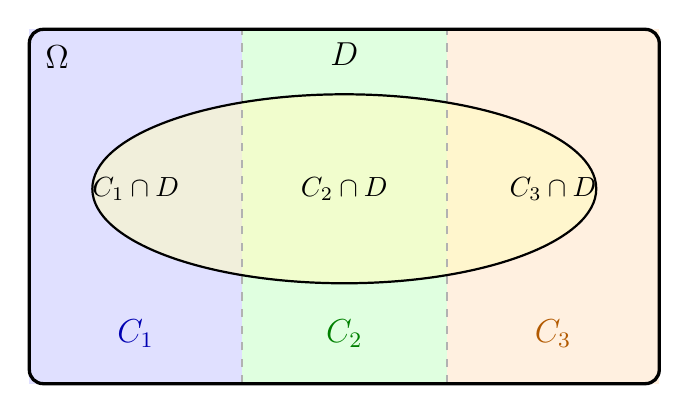
\begin{tikzpicture}[font=\small]

% --- Dimensions ---
\def\W{8}
\def\H{4.5}
\def\xA{2.7}
\def\xB{5.3}

% --- Fond des trois bandes (partition) ---
\fill[blue!12]   (0,0) rectangle (\xA,\H);
\fill[green!12] (\xA,0) rectangle (\xB,\H);
\fill[orange!12]  (\xB,0) rectangle (\W,\H);

% --- Ellipse D (remplie par-dessus) ---
\fill[yellow!25, opacity=0.55]
    (0.5*\W, 0.55*\H) ellipse [x radius=3.2, y radius=1.2];

% --- Frontières de la partition (par-dessus D) ---
\draw[thick, dashed, gray!60] (\xA,0) -- (\xA,\H);
\draw[thick, dashed, gray!60] (\xB,0) -- (\xB,\H);

% --- Contour de D ---
\draw[thick] (0.5*\W, 0.55*\H) ellipse [x radius=3.2, y radius=1.2];

% --- Cadre Omega ---
\draw[very thick, rounded corners=5pt] (0,0) rectangle (\W,\H);

% --- Étiquettes des régions ---
\node[font=\normalsize] at (0.5*\xA, 0.55*\H)         {$C_1\cap D$};
\node[font=\normalsize] at (0.5*\xA+0.5*\xB, 0.55*\H) {$C_2\cap D$};
\node[font=\normalsize] at (0.5*\xB+0.5*\W, 0.55*\H)  {$C_3\cap D$};

% --- Étiquettes principales (hors ellipse) ---
\node[font=\large, blue!70!black]   at (0.5*\xA, 0.14*\H)         {$C_1$};
\node[font=\large, green!50!black] at (0.5*\xA+0.5*\xB, 0.14*\H) {$C_2$};
\node[font=\large, orange!70!black]  at (0.5*\xB+0.5*\W, 0.14*\H)  {$C_3$};

% --- Étiquette D ---
\node[font=\large] at (0.5*\W, 0.93*\H) {$D$};

% --- Étiquette Omega ---
\node[anchor=north west, font=\large] at (0.08,\H-0.08) {$\Omega$};

\end{tikzpicture}
\end{solution}
\vspace{3.5cm}

\part[6] Quelle est la probabilité qu'une puce prise au hasard soit défectueuse?

\begin{solution}
Par la loi des probabilités totales,
\[
\mathbb{P}(D) = \mathbb{P}(D\mid C_1)\mathbb{P}(C_1) + \mathbb{P}(D\mid C_2)\mathbb{P}(C_2) + \mathbb{P}(D\mid C_3)\mathbb{P}(C_3).
\]
\[
\mathbb{P}(D) = 0{,}02\times 0{,}5 + 0{,}03\times 0{,}3 + 0{,}05\times 0{,}2 = 0{,}01+0{,}009+0{,}01 = 0{,}029.
\]
\[
\boxed{\mathbb{P}(D) = 0{,}029.}
\]
\end{solution}

\vspace{5cm}

\part[6] Si une puce choisie au hasard est défectueuse, quelle est la probabilité qu'elle provienne de la chaîne 3?

\begin{solution}
Par le théorème de Bayes,
\[
\mathbb{P}(C_3\mid D) = \frac{\mathbb{P}(D\mid C_3)\mathbb{P}(C_3)}{\mathbb{P}(D)} = \frac{0{,}05\times 0{,}2}{0{,}029} = \frac{0{,}01}{0{,}029}.
\]
\[
\boxed{\mathbb{P}(C_3\mid D) = \frac{10}{29} \approx 0{,}345.}
\]
\end{solution}

\vfill

\part \begin{subparts}
\subpart[1] Les événements \(C_1\), \(C_2\) et \(C_3\) forment une partition de l'espace échantillonnal.

\begin{oneparcheckboxes}
\correctchoice Vrai
\choice Faux
\end{oneparcheckboxes}

\subpart[1] Les événements \(C_1\) et \(D\) sont indépendants.

\begin{oneparcheckboxes}
\choice Vrai
\correctchoice Faux
\end{oneparcheckboxes}

\subpart[1] Les événements \(C_1\) et \(D\) sont mutuellement exclusifs.

\begin{oneparcheckboxes}
\choice Vrai
\correctchoice Faux
\end{oneparcheckboxes}
\end{subparts}
\vspace{0.5cm}
\end{parts}

\pageblanche

%%%%%%%%%%%%%%%% QUESTION MODULE 2 - VARIABLE ALÉATOIRE CONTINUE %%%%%%%%%%%%%%%%

\question[]\label{densitetriangle} Soit \(X\) une variable aléatoire continue de densité \(f_X\) définie par
\[
f_X(x) = \begin{cases}
kx & \text{si } 0 \le x < 2,\\
k(4-x) & \text{si } 2 \le x \le 4,\\
0 & \text{sinon.}
\end{cases}
\]

\begin{parts}
\part[4] Trouvez la valeur de \(k\).

\begin{solution}
On veut que l'aire totale sous la courbe vaille 1 :
\[
1 = \int_0^2 kx\,dx + \int_2^4 k(4-x)\,dx = k\left[\frac{x^2}{2}\right]_0^2 + k\left[4x-\frac{x^2}{2}\right]_2^4.
\]
\[
1 = k(2) + k\big[(16-8)-(8-2)\big] = 2k + 2k = 4k.
\]
\[
\boxed{k = \frac{1}{4}.}
\]
\end{solution}

\vspace{5cm}

\part[5] Calculez \(\mathbb{P}(1 < X < 3)\).

\begin{solution}
\begin{align*}
\mathbb{P}(1<X<3) &= \int_1^2 \frac{1}{4}x\,dx + \int_2^3 \frac{1}{4}(4-x)\,dx\\
&= \frac{1}{4}\left[\frac{x^2}{2}\right]_1^2 + \frac{1}{4}\left[4x-\frac{x^2}{2}\right]_2^3\\
&= \frac{1}{4}(2-0{,}5) + \frac{1}{4}\big[(12-4{,}5)-(8-2)\big]\\
&= 0{,}375 + 0{,}375 = 0{,}75.
\end{align*}
\end{solution}

\vfill

\pagesuivante{\ref{densitetriangle}}

\part[5] Calculez \(\mathbb{E}(X)\).

\begin{solution}
\begin{align*}
\mathbb{E}(X) &= \int_0^2 x\cdot\frac{1}{4}x\,dx + \int_2^4 x\cdot\frac{1}{4}(4-x)\,dx\\
&= \frac{1}{4}\left[\frac{x^3}{3}\right]_0^2 + \frac{1}{4}\left[2x^2-\frac{x^3}{3}\right]_2^4\\
&= \frac{1}{4}\cdot\frac{8}{3} + \frac{1}{4}\left[\left(32-\frac{64}{3}\right)-\left(8-\frac{8}{3}\right)\right]\\
&= \frac{2}{3} + \frac{1}{4}\left(\frac{32}{3}-\frac{16}{3}\right) = \frac{2}{3}+\frac{4}{3} = 2.
\end{align*}
\textit{Remarque : ce résultat était prévisible par symétrie de la densité autour de \(x=2\).}
\end{solution}
\end{parts}

\pageblanche

%%%%%%%%%%%%%%%% QUESTION MODULE 3 - LOIS DISCRÈTES %%%%%%%%%%%%%%%%

\question[]

\begin{parts}
\part[5] Un lot de \(20\) composantes électroniques contient \(5\) composantes défectueuses. On prélève, sans remise, un échantillon de \(4\) composantes. Quelle est la probabilité que l'échantillon contienne \emph{exactement une} composante défectueuse?

\begin{solution}
Soit \(X\) le nombre de composantes défectueuses dans l'échantillon. Comme le tirage se fait sans remise dans une population finie composée de deux catégories, \(X\) suit une loi hypergéométrique.
\[
\mathbb{P}(X=1) = \frac{\binom{5}{1}\binom{15}{3}}{\binom{20}{4}} = \frac{5\times 455}{4845} = \frac{2275}{4845} = \frac{455}{969}.
\]
\[
\boxed{\mathbb{P}(X=1) = \frac{455}{969} \approx 0{,}470.}
\]
\end{solution}

\vspace{5cm}

\part[5] Une entreprise de messagerie estime que \(8\%\) de ses colis sont livrés en retard, indépendamment les uns des autres. On sélectionne au hasard \(15\) colis. Quelle est la probabilité qu'\emph{au plus deux} colis parmi les \(15\) soient livrés en retard?

\begin{solution}
Soit \(Y\) le nombre de colis en retard parmi les \(15\). Alors \(Y \sim \text{Bin}(15;\,0{,}08)\).
\[
\mathbb{P}(Y\le 2) = \sum_{k=0}^{2}\binom{15}{k}(0{,}08)^k(0{,}92)^{15-k}.
\]
\[
\mathbb{P}(Y=0) = (0{,}92)^{15} \approx 0{,}2863,
\]
\[
\mathbb{P}(Y=1) = 15(0{,}08)(0{,}92)^{14} \approx 0{,}3735,
\]
\[
\mathbb{P}(Y=2) = \binom{15}{2}(0{,}08)^2(0{,}92)^{13} \approx 0{,}2273.
\]
\[
\boxed{\mathbb{P}(Y\le 2) \approx 0{,}2863+0{,}3735+0{,}2273 = 0{,}8871.}
\]
\end{solution}

\vfill

\part \begin{subparts}
\subpart[3] Une représentante commerciale conclut une vente avec probabilité \(p=0{,}25\) à chaque appel, indépendamment des autres appels. Quelle est la probabilité que sa première vente survienne exactement au \(4^\text{e}\) appel?

\begin{solution}
Le nombre d'appels avant la première vente suit une loi géométrique de paramètre \(p=0{,}25\).
\[
\mathbb{P}(X=4) = (0{,}75)^3(0{,}25) \approx 0{,}1055.
\]
\end{solution}

\vspace{4cm}

\subpart[3] En moyenne, combien d'appels devra-t-elle faire pour obtenir \(5\) ventes?

\begin{solution}
Le nombre d'appels nécessaires pour obtenir \(r=5\) succès suit une loi de Pascal (binomiale négative) de paramètre \(p=0{,}25\). L'espérance du nombre d'essais est
\[
\mathbb{E}(\text{appels}) = \frac{r}{p} = \frac{5}{0{,}25} = 20.
\]
\end{solution}
\end{subparts}
\end{parts}

\pageblanche

%%%%%%%%%%%%%%%% QUESTION MODULE 4 - LOIS CONTINUES / PROCESSUS DE POISSON %%%%%%%%%%%%%%%%

\question[]

Le temps entre deux pannes successives d'une machine industrielle suit une loi exponentielle d'espérance \(50\) heures.

\begin{parts}
\part[4] Quelle est la probabilité qu'aucune panne ne survienne au cours des \(20\) prochaines heures?

\begin{solution}
Le taux est \(\lambda = 1/50 = 0{,}02\) par heure. Soit \(X\) le temps avant la prochaine panne, \(X\sim\text{Exp}(0{,}02)\).
\[
\mathbb{P}(X>20) = e^{-0{,}02\times 20} = e^{-0{,}4} \approx 0{,}6703.
\]
\end{solution}

\vspace{4cm}

\part[4] Sachant qu'aucune panne n'est survenue au cours des \(20\) dernières heures, quelle est la probabilité qu'il n'y en ait pas non plus au cours des \(10\) prochaines heures?

\begin{solution}
La loi exponentielle est sans mémoire, donc
\[
\mathbb{P}(X>30\mid X>20) = \mathbb{P}(X>10) = e^{-0{,}02\times 10} = e^{-0{,}2} \approx 0{,}8187.
\]
\end{solution}

\vspace{4cm}

\part[6] En moyenne, combien de temps faudra-t-il attendre avant d'observer \(4\) pannes?

\begin{solution}
Le temps nécessaire pour observer \(k=4\) pannes suit une loi gamma de paramètre de forme \(k=4\) et de taux \(\lambda = 0{,}02\). L'espérance vaut
\[
\mathbb{E}(\text{temps}) = \frac{k}{\lambda} = \frac{4}{0{,}02} = 200 \text{ heures.}
\]
\end{solution}

\pagebreak

Une chaîne de production remplit des sacs de farine dont le poids \(X\) suit une loi normale d'espérance \(\mu = 1000\) g et de variance \(\sigma^2 = 225\) g\(^2\). On prélève un échantillon aléatoire de \(36\) sacs.

\part[4] Quelle est la probabilité que le poids moyen de l'échantillon soit inférieur à \(995\) g?

\begin{solution}
\(\overline{X}\sim\mathcal{N}\left(1000;\,\dfrac{225}{36}\right) = \mathcal{N}(1000;\,6{,}25)\), donc l'écart-type de \(\overline{X}\) est \(2{,}5\).
\begin{align*}
\mathbb{P}(\overline{X}<995) &= \mathbb{P}\left(\frac{\overline{X}-1000}{2{,}5} < \frac{995-1000}{2{,}5}\right)\\
&= \mathbb{P}(Z<-2) = 0{,}0228.
\end{align*}
\end{solution}

\vspace{4cm}

\part[4] Si l'on ignorait que \(X\) suit une loi normale, mais que l'on savait tout de même que \(\mathbb{E}(X)=1000\) et \(V(X)=225\), pourrait-on tout de même approximer la probabilité calculée en (d)? Expliquez votre réponse.

\begin{solution}
Oui. Puisque \(n=36\) est suffisamment grand, le théorème central limite (TCL) permet d'approximer la loi de \(\overline{X}\) par une loi normale d'espérance \(1000\) et de variance \(225/36\), peu importe la loi exacte de \(X\). Le calcul et la réponse numérique de la partie (d) demeurent donc valides en approximation.
\end{solution}
\end{parts}

\pageblanche

%%%%%%%%%%%%%%%% QUESTION MODULE 5 - LOI CONJOINTE %%%%%%%%%%%%%%%%

\question Deux tests de dépistage, A et B, sont effectués sur des échantillons d'eau. On définit \(X\) le nombre de contaminants détectés par le test A (\(0\), \(1\) ou \(2\)) et \(Y\) le résultat du test B (\(0\) = négatif, \(1\) = positif).

Voici la fonction de probabilité conjointe de \(X\) et \(Y\).

\begin{center}
\begin{tabular}{cc|cc|c}
$p(x,y)$ & & \multicolumn{2}{c|}{$y$} & \\
 & & $0$ & $1$ & \\
\hline
 & $0$ & $0{,}10$ & $0{,}05$ & \\
$x$ & $1$ & $0{,}15$ & $0{,}25$ & \\
 & $2$ & $0{,}15$ & $0{,}30$ & \\
\hline
\end{tabular}
\end{center}

\begin{parts}
\part[4] Donnez la loi marginale de \(X\).

\begin{solution}
On somme chaque ligne du tableau :
\[
p_X(0) = 0{,}10+0{,}05 = 0{,}15,\qquad p_X(1) = 0{,}15+0{,}25 = 0{,}40,\qquad p_X(2) = 0{,}15+0{,}30 = 0{,}45.
\]
On vérifie que \(0{,}15+0{,}40+0{,}45 = 1\).
\end{solution}

\vspace{3cm}

\part[4] Calculez \(\mathbb{E}(Y)\).

\begin{solution}
La loi marginale de \(Y\) est \(p_Y(0) = 0{,}10+0{,}15+0{,}15 = 0{,}40\) et \(p_Y(1) = 0{,}05+0{,}25+0{,}30 = 0{,}60\).
\[
\mathbb{E}(Y) = 0\times 0{,}40 + 1\times 0{,}60 = 0{,}6.
\]
\end{solution}

\vspace{3cm}

\part[4] Sachant que \(\mathbb{E}(X) = 1{,}3\), calculez la covariance entre \(X\) et \(Y\).

\begin{solution}
On calcule d'abord \(\mathbb{E}(XY)\) :
\[
\mathbb{E}(XY) = (0)(0)(0{,}10)+(0)(1)(0{,}05)+(1)(0)(0{,}15)+(1)(1)(0{,}25)+(2)(0)(0{,}15)+(2)(1)(0{,}30).
\]
\[
\mathbb{E}(XY) = 0{,}25 + 0{,}60 = 0{,}85.
\]
Ainsi,
\[
\text{Cov}(X,Y) = \mathbb{E}(XY) - \mathbb{E}(X)\mathbb{E}(Y) = 0{,}85 - (1{,}3)(0{,}6) = 0{,}85-0{,}78 = 0{,}07.
\]
\end{solution}

\vfill

\part Les variables aléatoires \(X\) et \(Y\) sont indépendantes. \textit{Une réponse sans bonne justification n'aura aucun point, même si elle est bonne.}

\begin{oneparcheckboxes}
\choice Vrai
\correctchoice Faux
\end{oneparcheckboxes}

\textbf{Justification:}
\begin{solution}
Il suffit de trouver une combinaison où \(p(x,y)\neq p_X(x)p_Y(y)\). Par exemple, \(p(0,0)=0{,}10\) alors que \(p_X(0)p_Y(0) = (0{,}15)(0{,}40) = 0{,}06 \neq 0{,}10\). De plus, \(\text{Cov}(X,Y)=0{,}07\neq 0\), ce qui confirme que \(X\) et \(Y\) ne sont pas indépendantes.
\end{solution}
\vspace{3cm}
\end{parts}

\pageblanche

%%%%%%%%%%%%%%%% QUESTION MODULE 6 - STATISTIQUE DESCRIPTIVE %%%%%%%%%%%%%%%%

\question[]

On mesure le temps de réponse (en millisecondes) d'un serveur pour \(9\) requêtes :
\[
12,\ 15,\ 14,\ 22,\ 13,\ 19,\ 14,\ 100,\ 16.
\]

\begin{parts}
\part[3] Calculez la moyenne et la médiane échantillonnales. Expliquez pourquoi elles sont si différentes.

\begin{solution}
En ordonnant l'échantillon :
\[
12,\ 13,\ 14,\ 14,\ 15,\ 16,\ 19,\ 22,\ 100.
\]
La moyenne est
\[
\overline{x} = \frac{12+13+14+14+15+16+19+22+100}{9} = \frac{225}{9} = 25.
\]
Comme \(n=9\) est impair, la médiane est la \(5^\text{e}\) observation ordonnée :
\[
\tilde{x} = 15.
\]
La moyenne est beaucoup plus grande que la médiane car la valeur \(100\) est une observation extrême qui tire la moyenne vers le haut, alors que la médiane, étant une mesure robuste, n'est pas affectée par cette valeur.
\end{solution}

\vspace{4cm}

\part[4] Calculez le premier quartile \(Q_1\), le troisième quartile \(Q_3\) et l'écart interquartile (EIQ).

\begin{solution}
La médiane divise l'échantillon ordonné en deux moitiés (en excluant la valeur centrale) :
\[
\text{moitié inférieure : } 12,\,13,\,14,\,14 \qquad \text{moitié supérieure : } 16,\,19,\,22,\,100.
\]
\[
Q_1 = \frac{13+14}{2} = 13{,}5, \qquad Q_3 = \frac{19+22}{2} = 20{,}5.
\]
\[
\text{EIQ} = Q_3-Q_1 = 20{,}5-13{,}5 = 7.
\]
\end{solution}

\vspace{4cm}

\part[3] Calculez les bornes théoriques \(b_{\text{inf}}\) et \(b_{\text{sup}}\) utilisées pour la construction du diagramme en boîte, et déterminez si la valeur \(100\) doit être considérée comme une valeur aberrante.

\begin{solution}
\[
b_{\text{inf}} = Q_1 - 1{,}5\,\text{EIQ} = 13{,}5 - 10{,}5 = 3,
\]
\[
b_{\text{sup}} = Q_3 + 1{,}5\,\text{EIQ} = 20{,}5 + 10{,}5 = 31.
\]
Puisque \(100 > b_{\text{sup}} = 31\), la valeur \(100\) est considérée comme une valeur aberrante et serait représentée par un point isolé sur le diagramme en boîte, la moustache supérieure s'arrêtant à la plus grande valeur inférieure ou égale à \(31\), soit \(22\).
\end{solution}

\end{parts}

\pageblanche
\end{questions}
\end{document}